\documentclass{cheatsheet}
\usepackage{enumitem}
\begin{document}

\section{ECE 174: Midterm}
\section{\normalsize Brandon Szeto}
\section{\normalsize PID: A17002478}

\vspace{2mm}

\hrule

\vspace{5mm}

\footnotesize

% Lecture 10/03
% Vector addition, scalar multiplication over vector spaces R^n and R^nxm
% Subspaces defined using vector spaces

\section{\small Properties:}
\[
	\mathbb{R}^n =
	\left\{
	\begin{bmatrix}
		x_1    \\
		x_2    \\
		\vdots \\
		x_n
	\end{bmatrix},
	x_1, x_2, \dots, x_n \in \mathbb{R}
	\right\}
\]
Here, $\mathbb{R}^n$ is the set of \textit{all possible} real-valued $n$-tuples
(depicted as column vectors) which must be closed under vector addition and
scalar multiplication. \\

\section{\small Vector addition:}
 ($\mathbb{R}^n \times \mathbb{R}^n \rightarrow \mathbb{R}^n$):
\[
	x =
	\begin{bmatrix}
		x_1    \\
		\vdots \\
		x_n
	\end{bmatrix} \in \mathbb{R}^n,
	y =
	\begin{bmatrix}
		y_1    \\
		\vdots \\
		y_n
	\end{bmatrix} \in \mathbb{R}^n
\]
\[
	x + y =
	\begin{bmatrix}
		x_1 + y_1 \\
		\vdots    \\
		x_n + y_n
	\end{bmatrix} \in \mathbb{R}^n
\]

\section{\small Scalar multiplication}
 ($\mathbb{R} \times \mathbb{R}^n \rightarrow \mathbb{R}^n$)
\[
	x =
	\begin{bmatrix}
		x_1    \\
		\vdots \\
		x_n
	\end{bmatrix} \in \mathbb{R}^n,
	\alpha \in \mathbb{R}
\]
\[
	\alpha \cdot x =
	\begin{bmatrix}
		\alpha \cdot x_1 \\
		\vdots           \\
		\alpha \cdot x_n
	\end{bmatrix} \in \mathbb{R}^n
\]

% \textbf{Properties:}
% \begin{enumerate}
% 	\item $\mathbb{R}^n$ is closed under vector addition and scalar
% 	      multiplication.
% 	\item $\vec{x} + \vec{y} = \vec{y} + \vec{x} \quad \forall \vec{x}, \vec{y} \in
% 		      \mathbb{R}^n$
% 	\item $(\vec{x} + \vec{y}) + \vec{z} = \vec{x} + (\vec{y} + \vec{z}) \quad
% 		      \forall \vec{x}, \vec{y}, \vec{z} \in \mathbb{R}^n$
% 	\item $\alpha(\beta \vec{x}) = (\alpha \beta) \vec{x} \quad \forall \vec{x} \in \mathbb{R}^n, \alpha, \beta \in \mathbb{R}$
% 	\item $\alpha \cdot (\vec{x} + \vec{y}) = \alpha \vec{x} + \alpha \vec{y} \quad \forall \vec{x}, \vec{y} \in \mathbb{R}^n, \alpha \in \mathbb{R}$
% 	\item $(\alpha + \beta) \vec{x} = \alpha \vec{x} + \beta \vec{x} \quad \forall \vec{x} \in \mathbb{R}^n, \alpha, \beta \in \mathbb{R}$
% 	\item $1 \cdot \vec{x} = \vec{x} \quad \forall \vec{x} \in \mathbb{R}^n$
% 	\item $0 \cdot \vec{x} = \vec{0} \quad \forall \vec{x} \in \mathbb{R}^n$
% 	\item For every $\vec{x} \in \mathbb{R}^n$, there exists a unique vector
% 	      $\vec{x}_I \in \mathbb{R}^n$ such that $\vec{x} + \vec{x}_I = \vec{0}$
% \end{enumerate}

$\mathbb{R}^n$ and $\mathbb{R}^{n \times m}$ satisfies all the properties of
a vector space.

\section{\small Matrix-Matrix Multiplication}

You can multiply two matrices $ \mathbf{A} \in \mathbb{R}^{m \times p}$
and $\mathbf{A} \in \mathbb{R}^{p \times n}$. Then the product matrix
$\mathbf{C} = \mathbf{AB} \in \mathbb{R}^{m \times n}$ is defined as:
\[
	\mathbf{C}_{ij} = \sum_{k=1}^{p} \mathbf{A}_{ik} \mathbf{B}_{kj}
\]

\section{\small Transpose of a matrix}

The transpose of a matrix $\mathbf{A} \in \mathbb{R}^{m \times n}$, denoted by
$\mathbf{A}^T$, is defined as the matrix s.t. $\mathbf{A}^T_{ij} =
	\mathbf{A}_{ji} \forall i = 1 \ldots n, j = 1 \ldots m$. Properties include:

\begin{enumerate}[label=(\roman*)]
	\item $(\mathbf{A}^T)^T = \mathbf{A}$
	\item $(\mathbf{A} + \mathbf{B})^T = \mathbf{A}^T + \mathbf{B}^T$
	\item $(\mathbf{AB})^T = \mathbf{B}^T \mathbf{A}^T$
	\item $(\alpha \mathbf{A})^{T} = \alpha \mathbf{A}^T$
\end{enumerate}

\section{\small Trace}
The trace of an $n \times n$ matrix $\mathbf{A}$, denoted by
$\text{tr}(\mathbf{A})$, is defined as
\[
	\text{tr}(\mathbf{A}) = \sum_{i=1}^{n} \mathbf{A}_{ii}
\]
Properties include:
\begin{enumerate}[label=(\roman*)]
	\item $\text{tr}(\mathbf{A} + \mathbf{B}) = \text{tr}(\mathbf{A}) + \text{tr}(\mathbf{B})$
	\item $\text{tr}(\alpha \mathbf{A}) = \alpha \text{tr}(\mathbf{A})$
	\item $\text{tr}(\mathbf{AB}) = \text{tr}(\mathbf{BA})$
	\item $\text{tr}(\mathbf{A}^T) = \text{tr}(\mathbf{A})$
\end{enumerate}

\section{\small Invertible Matrices}
An $n \times n$ matrix $\mathbf{A}$ is invertible if there exists a matrix
$\mathbf{B}$ such that $\mathbf{AB} = \mathbf{BA} = \mathbf{I}_n$. If
$\mathbf{A}$ is invertible, the inverse of $\mathbf{A}$ is denoted by
$\mathbf{A}^{-1}$, and $\mathbf{A}^{-1} \mathbf{A} = \mathbf{A} \mathbf{A}^{-1}
	= \mathbf{I}_n$. $\mathbf{A}^{-1}$  can be calculated by $\mathbf{A}^{-1} =
	\frac{1}{\text{det}(\mathbf{A})} \text{adj}(\mathbf{A})$, where
$\text{adj}(\mathbf{A})$ is the adjugate matrix of $\mathbf{A}$ and
$\text{det}(\mathbf{A})$ is the determinant of $\mathbf{A}$.\\
\textbf{2x2 Matrix:}
Let $\mathbf{A} = \begin{bmatrix}
		a & b \\
		c & d
	\end{bmatrix}$. Then $\mathbf{A}^{-1} = \frac{1}{ad - bc} \begin{bmatrix}
		d  & -b \\
		-c & a
	\end{bmatrix}$


\section{\small Subspaces:}
A \textit{subspace} $S$ of $\mathbb{R}^n$ is a "non-empty" subset of
$\mathbb{R}^n$ with the following properties:
\begin{enumerate}[label=(\roman*)]
	\item If $\vec{u}, \vec{v} \in S$, then $\vec{u} + \vec{v} \in S$
	\item If $\vec{u} \in S$, then $\alpha \vec{u} \in S$ for all $\alpha \in \mathbb{R}$
\end{enumerate}
The zero vector of $\mathbb{R}^n$ \textit{must} be in $S$, and is a subspace in
it of itself.\\

A \textit{subspace} in $\mathbb{R}^n$ can only be:
\begin{enumerate}[label=(\roman*)]
	\item $\mathbb{R}^n$ itself ($n$-dimensional)
	\item $\{0\}$ (zero-dimensional)
	\item Subspaces of dimension $1, 2, \dots, n-1$
\end{enumerate}


% Lecture 10/05
% Subspaces
% Range

\section{\small Span:}

Suppose we are given $k$ vectors $\vec{v}_1, \vec{v}_2, \ldots, \vec{v}_k
	\in \mathbb{R}^n$. Then the \textbf{span} of these vectors is the set of
all linear combinations of these vectors.

\[
	\operatorname{span} \left\{ \vec{v}_1, \vec{v}_2, \ldots, \vec{v}_l \right\}
	=
\]
\[
	\sum_{i = 1}^k \alpha_i \vec{v}_i, \quad \alpha_i \ldots \alpha_k \in \mathbb{R}
\]

\section{\small Line:}
Given a vector $\vec{v}_0 \in \mathbb{R}^n$ define the following set:\\
$ \mathbb{L}_n := \{ \vec{x} \in \mathbb{R}^n, \text{s.t. } \vec{x} = \alpha
	\cdot \vec{v}_0 \text{ for some } \alpha \in \mathbb{R} \} $

$\mathbb{L}_n$ represents a line in $\mathbb{R}^n$. It is the span of a single
vector $\vec{v}_0$, is a subspace of $\mathbb{R}^n$, and has dimension 1.

\section{\small Range:}
Given $A \in \mathbb{R}^{m \times n}$ define the following set:
\[
	\begin{aligned}
		\mathcal{R}(A) : & = \left\{ \mathbb{A} \vec{x}, \quad \vec{x} \in \mathbb{R}^n
		\right\}                                                                        \\
		                 & = \left\{ \sum_{i = 1}^n \vec{a}_i\vec{x}_i, \vec{x}_i \in
		\mathbb{R} \right\}
	\end{aligned}
\]
We have
\[
	\mathcal{R}(A) = \operatorname{span} \left\{ \vec{a}_1, \vec{a}_2, \ldots, \vec{a}_n \right\}
\]
$R(A)$ represents the range of $A$. It is a subspace of $\mathbb{R}^m$.

\section{\small Null space:}
Given $A \in \mathbb{R}^{m \times n}$ define the following set:
\[
	\mathcal{N}(A) := \left\{ \vec{x} \in \mathbb{R}^n, \quad A \vec{x} = \vec{0} \right\}
\]


% Lecture 10/10
% Linear Independence
% Null space, Range
% Solving b = Ax

\section{\small Linear Independence}

A set of non-zero vectors $\{\vec{v}_1, \vec{v}_2, \dots, \vec{v}_k \in
	\mathbb{R}^n\}$ are said to be \textbf{linearly dependent} if there exists real
scalars $\alpha_1, \alpha_2, \dots, \alpha_k$ \textit{not all zero} such that:
\[
	\sum_{i=1}^{k} \alpha_i \vec{v}_i = \vec{0}
\]
In this case, we have $\mathcal{N}(V) \neq 0$.
Conversely, $\{\vec{v}_1, \vec{v}_2, \dots, \vec{v}_k \in \mathbb{R}^n\}$ are
\textbf{linearly independent} if the only solution to the equation:
\[
	\sum_{i=1}^{k} \alpha_i \vec{v}_i \leftrightarrow \alpha_1 = \alpha_2 =
	\ldots = \alpha_k =
	0
\]
In this case, we have $\mathcal{N}(V) = 0$.\\

Given $\vec{b} \in \mathbb{R}^m$, $\vec{x} \in \mathbb{R}^m$, and $\mathbf{A}
	\in \mathbb{R}^{n \times m}$, consider the equation $\mathbf{A} \vec{x} = \vec{b}$.

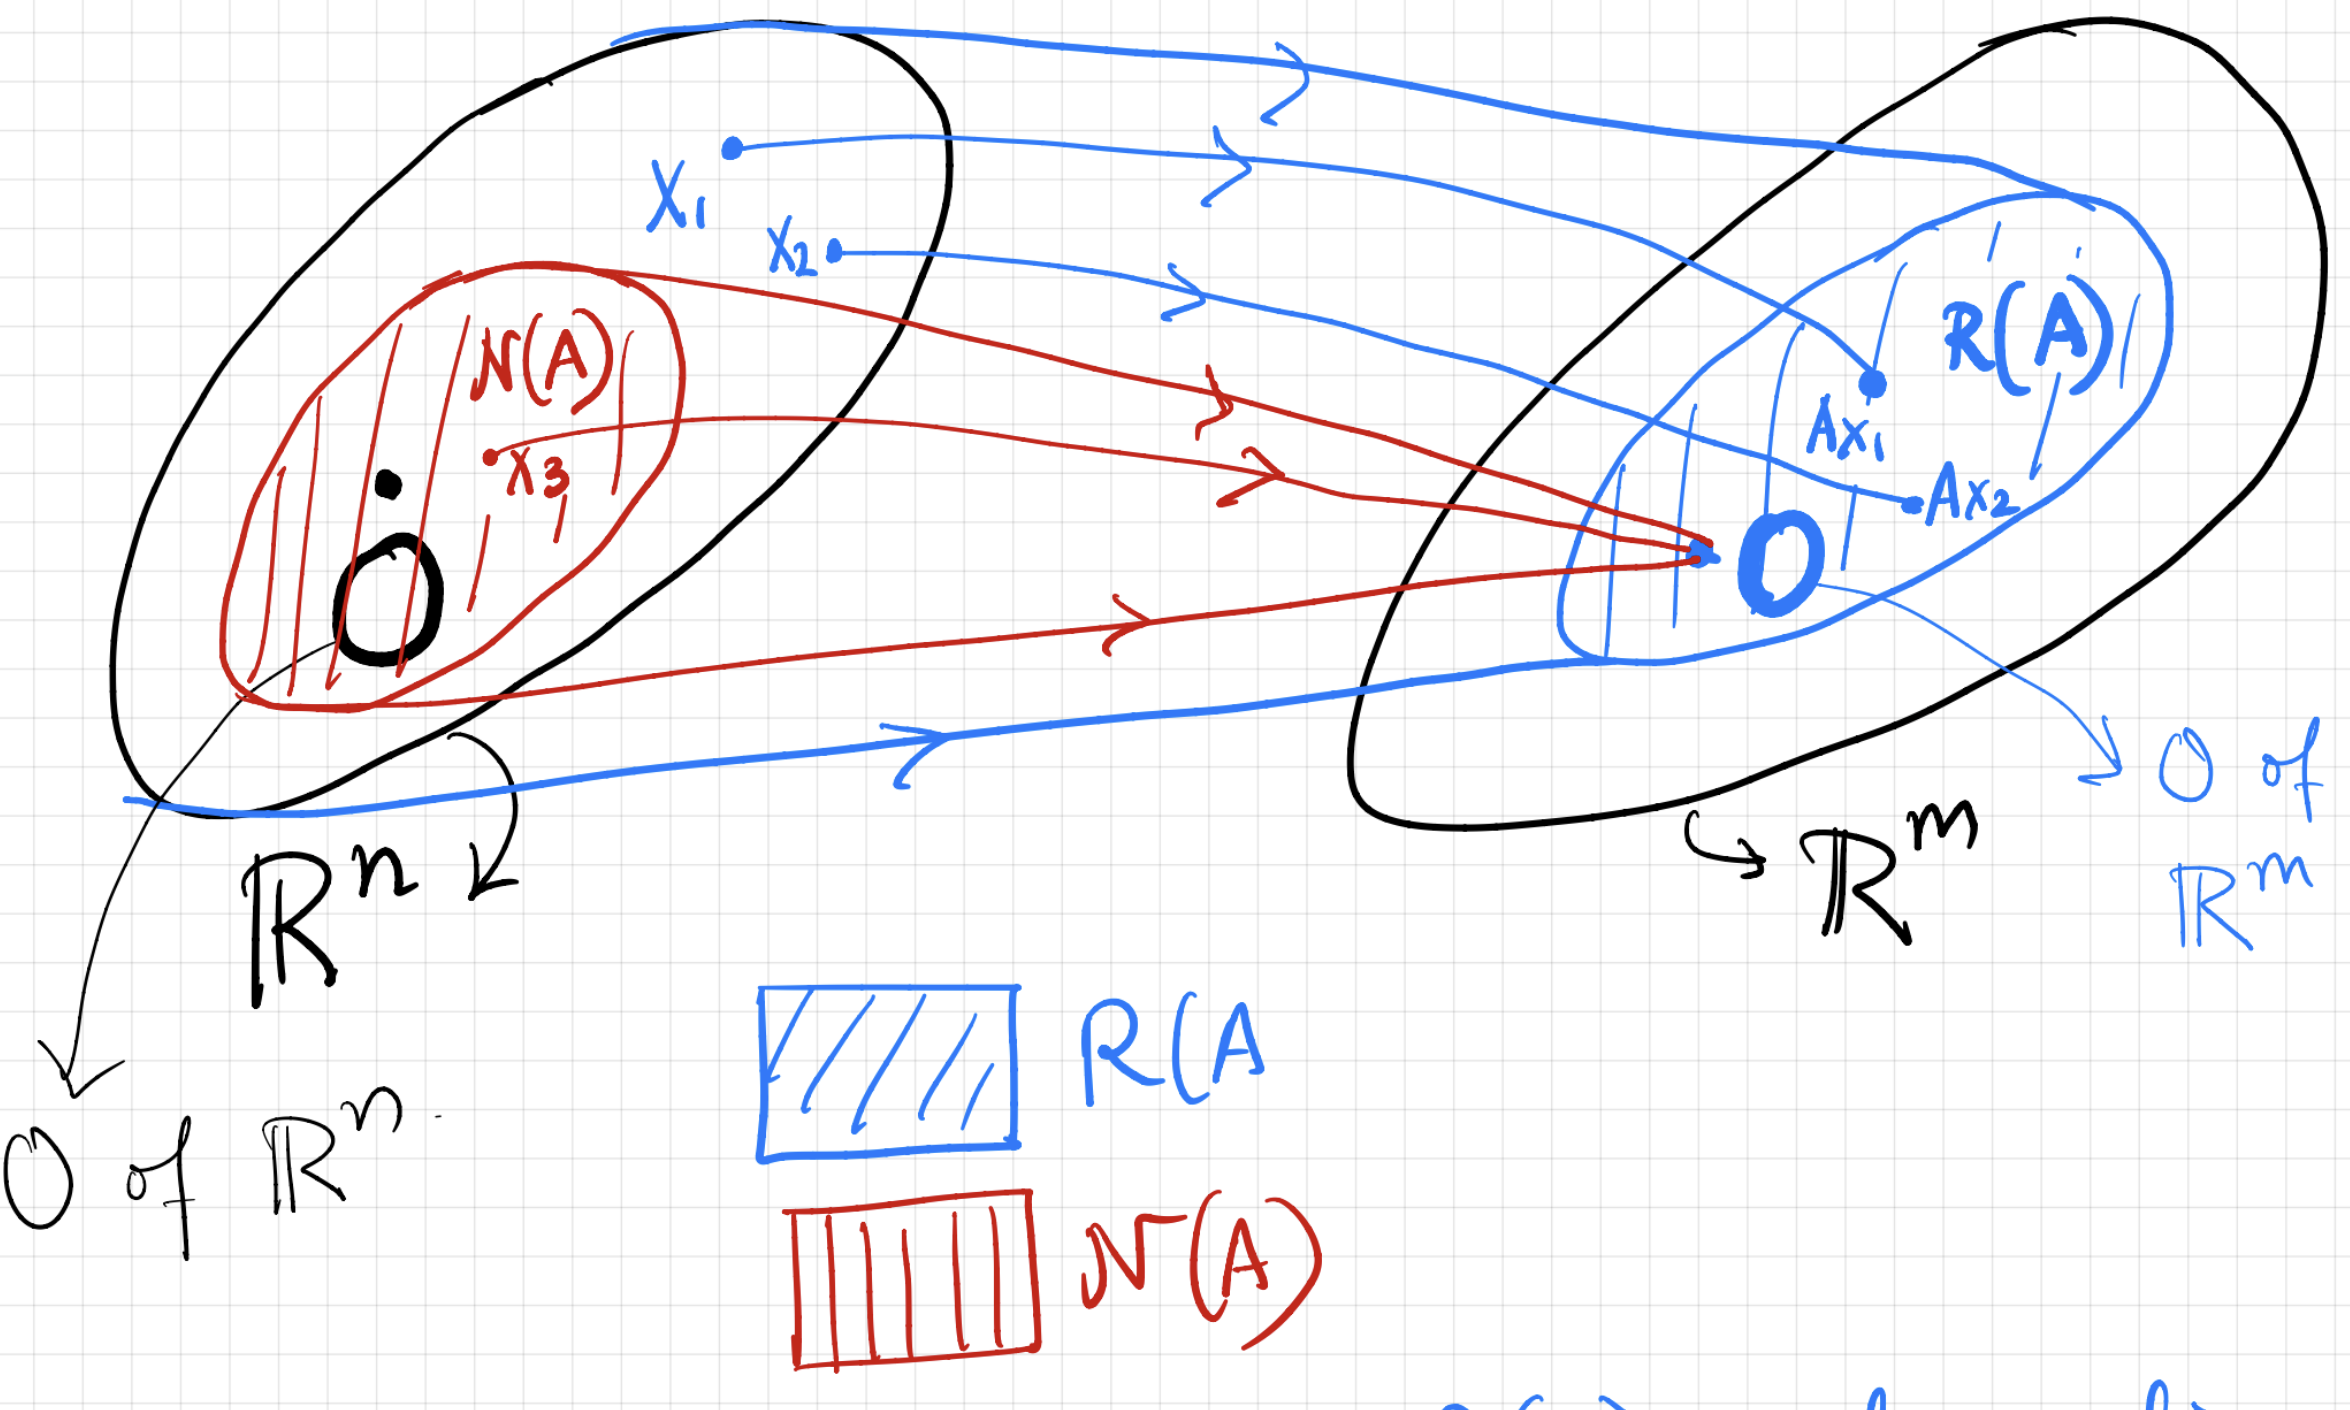
\includegraphics[width=0.2\textwidth]{images/RnRm2.png} \\

The entirety of $\mathbb{R}^n$ is mapped onto $\mathbb{R}^m$ by $\mathbf{A}$
($\vec{x}_k$ maps to $\mathbf{A} \vec{x}_k \in \mathbb{R}^m$). The entirety of
$\mathcal{N}(A) \in \mathbb{R}^n$ is mapped to $\vec{0} \in \mathbb{R}^m$.

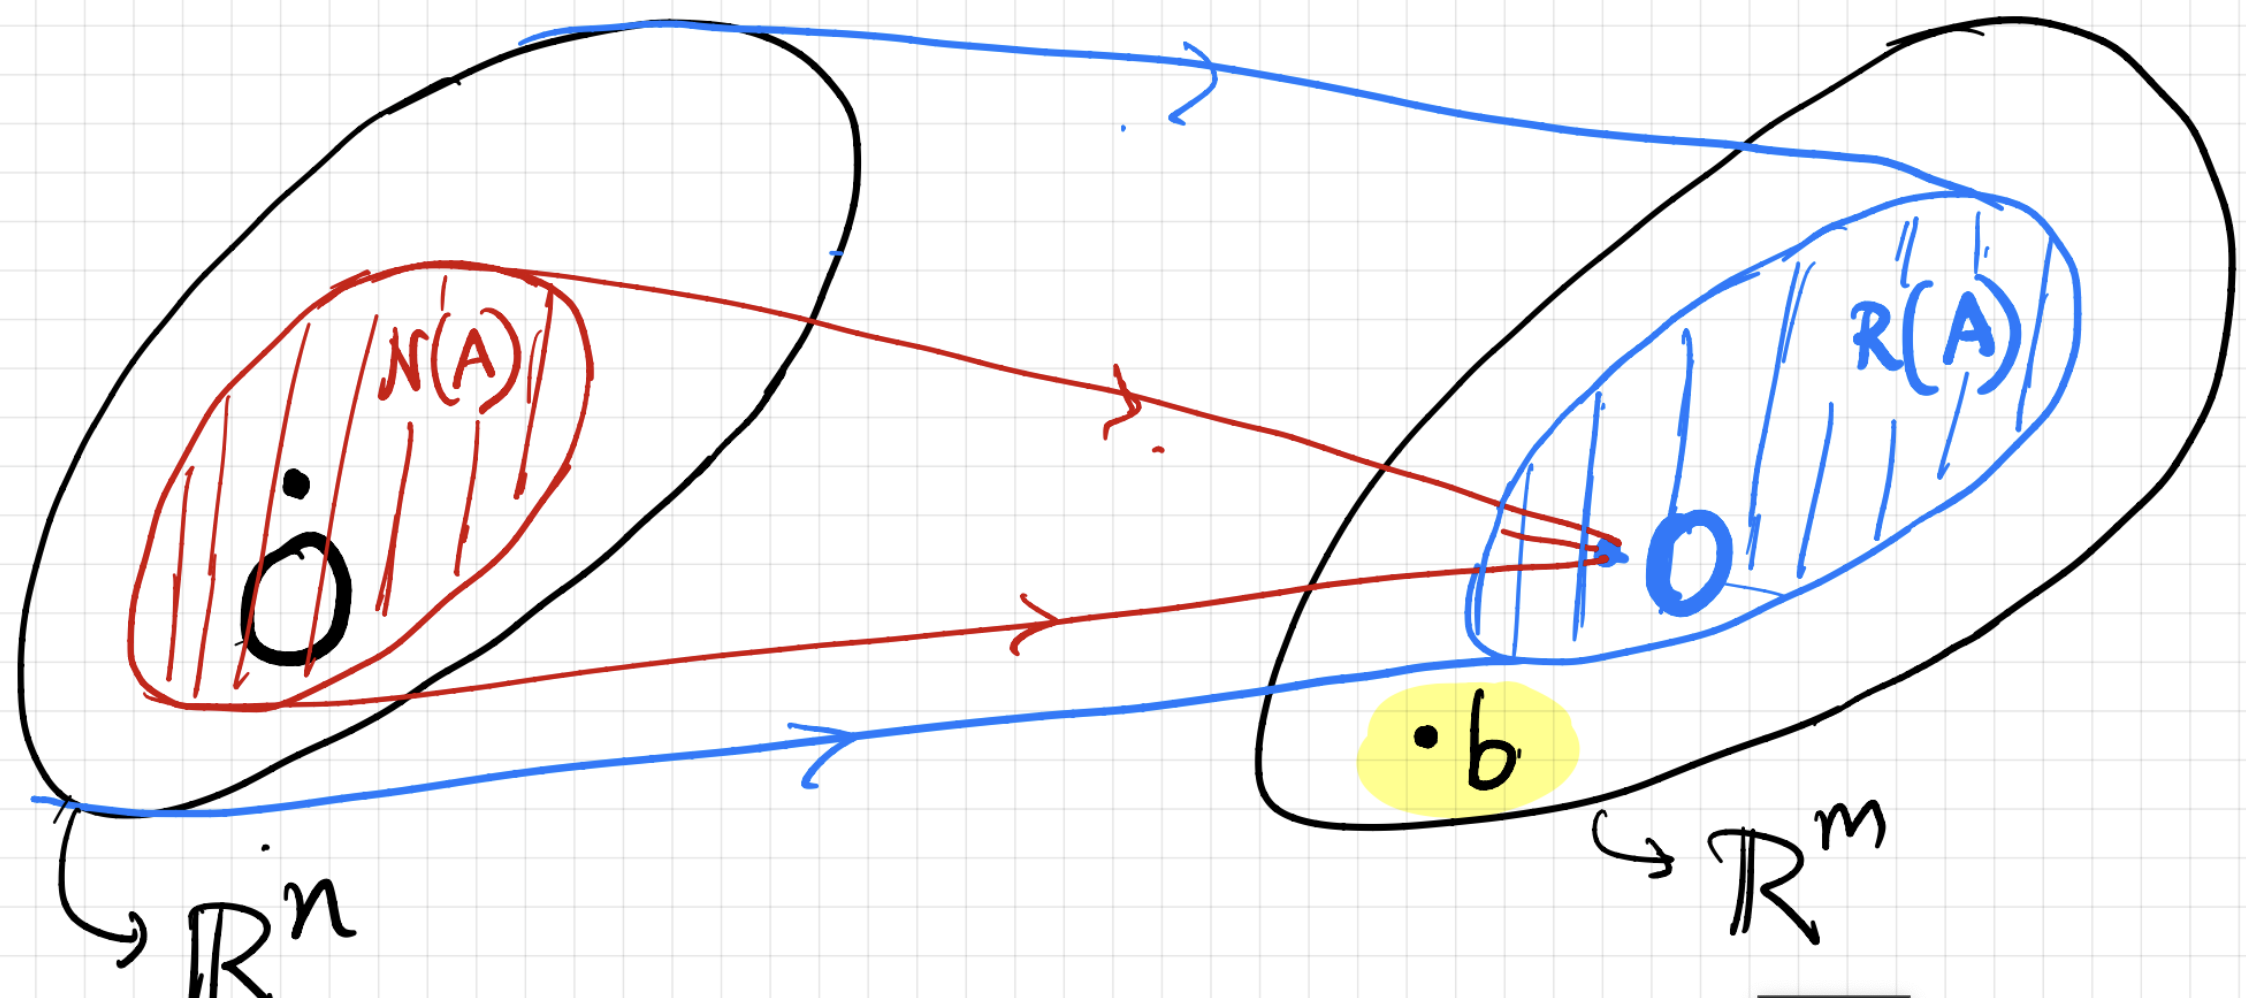
\includegraphics[width=0.2\textwidth]{images/RnRm.png} \\
Now consider $\vec{b}$ which may or may not belong to $\mathcal{R}(A)$. Then we
can use the following to determine the number of solutions:

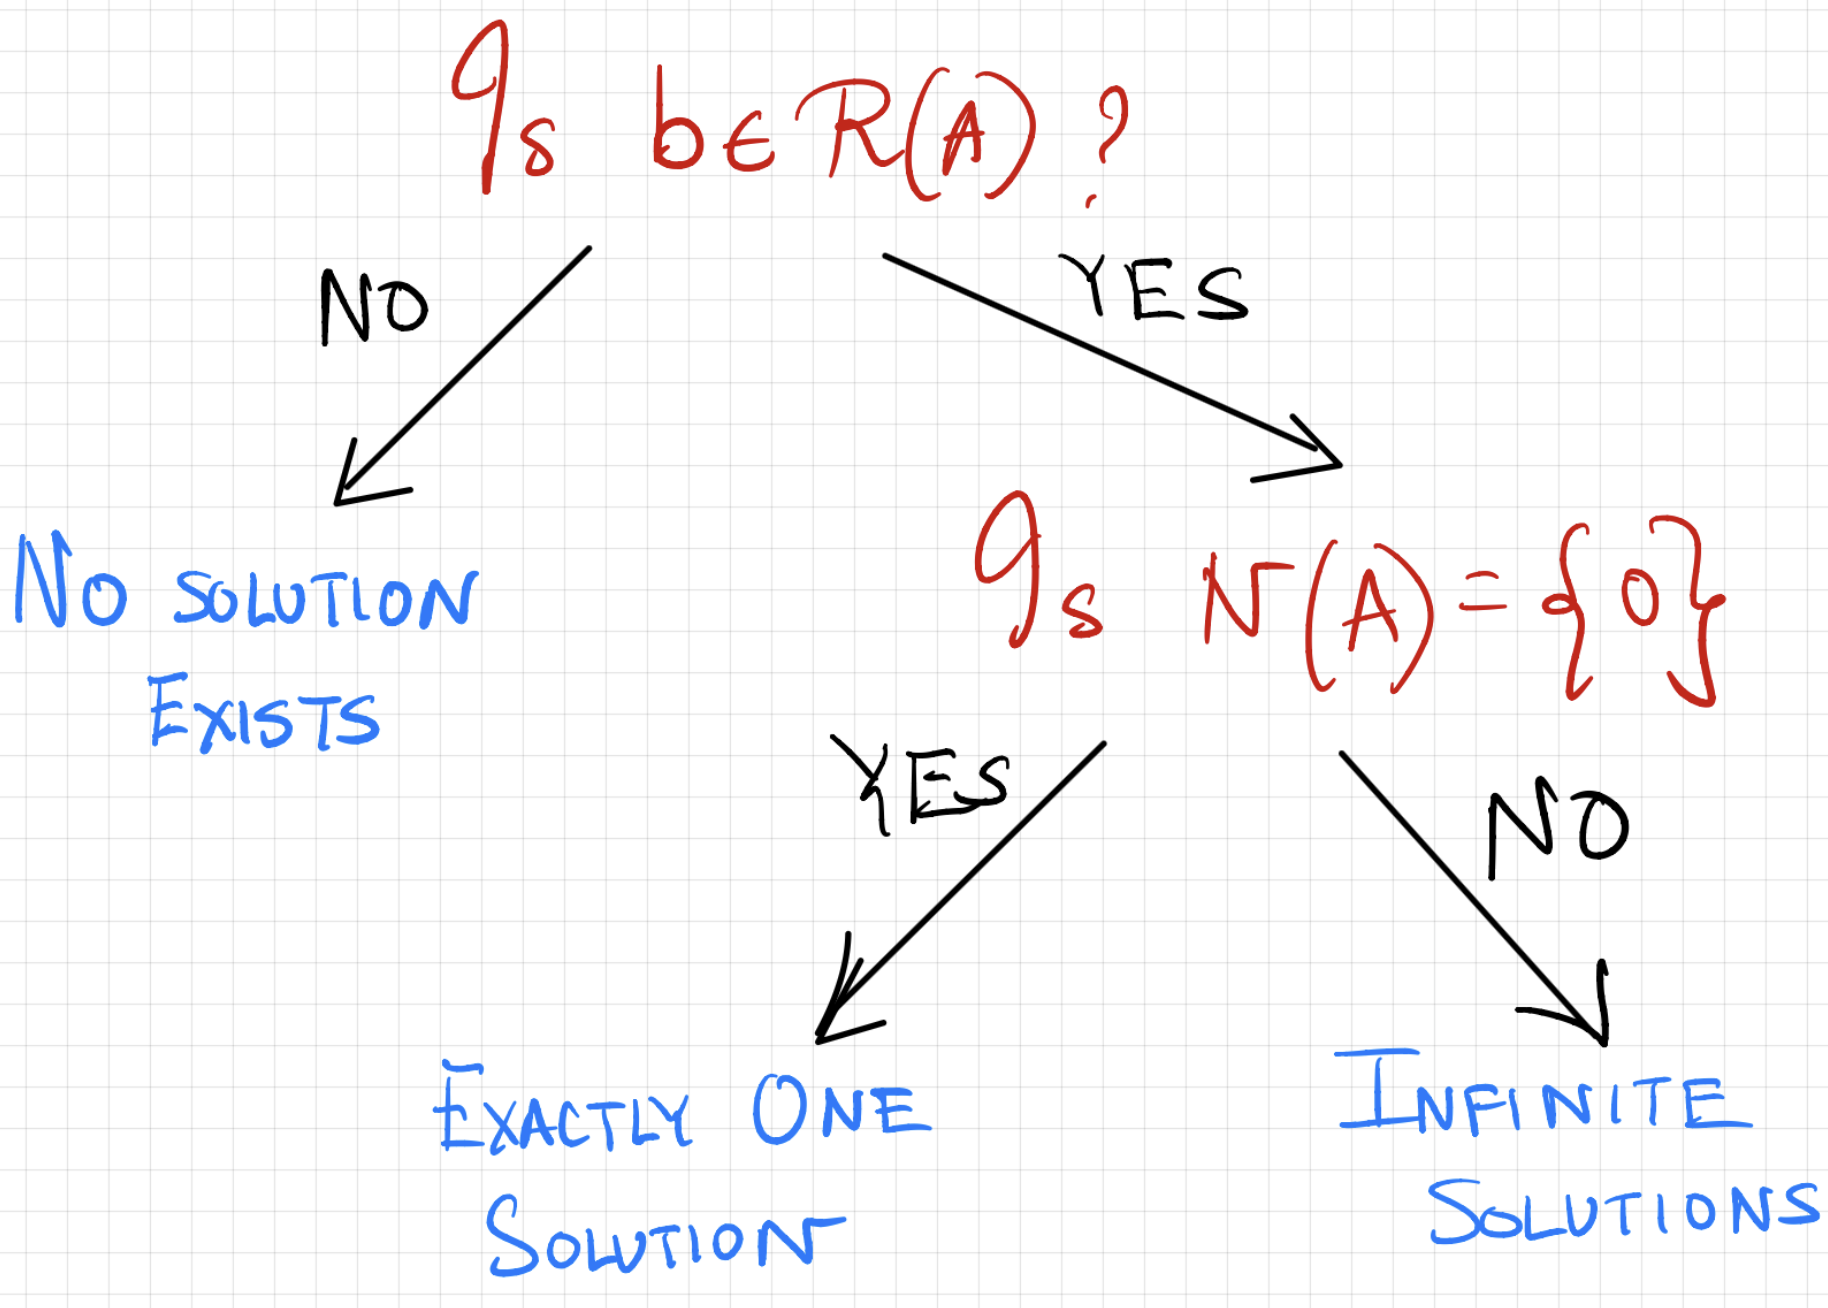
\includegraphics[width=0.2\textwidth]{images/full_picture.png}


\section{\small Basis}

Given a subspace $S$ of $\mathbb{R}^n$, a set of vectors $ \left\{
	\vec{v}_1, \vec{v}_2, \ldots, \vec{v}_k \right\}$ is a \textbf{basis} if:

\begin{enumerate}[label=(\roman*)]
	\item $\operatorname{span} \left\{ \vec{v}_1, \vec{v}_2, \ldots, \vec{v}_k
		      \right\} = S$ (i.e. every vector in $S$ can be written as a linear
	      combination of the vectors in the set)
	\item The vectors are linearly independent.
\end{enumerate}

1. Every subspace has a basis \\
2. Every basis of the same subspace of $\mathbb{R}^n$ has the same number of
elements (or cardinality)

\section{\small Basis Properties}

\textbf{Unique Representation:}\\
Let $S$ be a subspace and $\left\{ \vec{v}_1,
	\vec{v}_2, \ldots, \vec{v}_k \right\}$ be a basis for $S$. Then every vector
$\vec{v} \in S$ can be written \textit{uniquely} as a linear combination of
$\left\{ \vec{v}_1, \vec{v}_2, \ldots, \vec{v}_k \right\}$.

\textbf{Generating Bases:}\\
Let $\left\{ \vec{v}_1, \vec{v}_2, \ldots,
	\vec{v}_k \right\}$ be a basis of $\mathbb{R}^n$. Let $\mathbf{A} \in
	\mathbb{R}^{n \times n}$ be such that $\operatorname{rank} \mathbf{A} = n$.
Then $\left\{ \mathbf{A} \vec{v}_1, \mathbf{A} \vec{v}_2, \ldots, \mathbf{A}
	\vec{v}_n \right\}$ is also a basis of $\mathbb{R}^n$.

\textbf{Dimension-independence inequality:}\\
Let $S$ be a subspace of dimension $k$. Let $\left\{ \vec{v}_1, \vec{v}_2,
	\ldots, \vec{v}_p \right\}$ be a set of linearly independent vectors in $S$.
Then we must have $p \leq k$. \textbf{Corollary:} If we have a set of $k +
	1$ vectors, then they must be linearly dependent.

\section{\small Dimension}
The common cardinality shared by all bases of a subspace $S \in \mathbb{R}^n$ is
known as the \textit{dimension} of $S$. Can be thought of from the perspetive of
number of vectors in a linearly independent set (i.e. if there is no set of
linearly independent vectors with cardinality $k + 1$, then the dimension of the
set of vectors must be $k$.

\section{\small Some facts about bases}
\begin{enumerate}[label=(\roman*)]
	\item Every subspace of $\mathbb{R}^n$ has a basis
	\item Every basis of the same subspace of $\mathbb{R}^n$ has the same number of
	      elements (or cardinality)
	\item Let $S$ be a subspace and $\left\{ \vec{v}_1,
		      \vec{v}_2, \ldots, \vec{v}_k \right\}$ be a basis for $S$. Then
	      $\left\{ \alpha_1 \vec{v}_1, \alpha_2 \vec{v}_2, \ldots, \alpha_k
		      \vec{v}_k \right\}$ is a basis for $S$ for any $\alpha_1, \alpha_2,
		      \ldots \alpha_k \neq 0$.
\end{enumerate}


% Lecture 10/12
% Solving b = Ax
% Basis and dimension

% Lecture 10/17
% Basis and dimension examples
% Properties of bases

% Lecture 10/19
% Basis, dimensions, examples
% Properties of bases
% Linear maps: intro

\section{\small Example 1}

Consider the following set $S$ in $\mathbb{R}^3$:
\[
	S = \left\{
	\begin{bmatrix}
		x \\ y \\ z
	\end{bmatrix}
	\in \mathbb{R}^3
	\text{ s.t. }
	x - 2y = 0
	\right\}
\]
Let us construct a basis:
\[
	\begin{bmatrix}
		x \\ y \\ z
	\end{bmatrix} \in S
	\leftrightarrow
	x
	\begin{bmatrix}
		1 \\ \frac{1}{2} \\ 0
	\end{bmatrix} +
	z
	\begin{bmatrix}
		0 \\ 0 \\ 1
	\end{bmatrix}
\]
Any vector in $S$ can be written as a linear combination of the
two vectors above. Therefore, the two vectors form a basis for $S$.
\[
	S \subseteq \operatorname{span}\left\{
	\begin{bmatrix}
		1 \\ \frac{1}{2} \\ 0
	\end{bmatrix},
	\begin{bmatrix}
		0 \\ 0 \\ 1
	\end{bmatrix}
	\right\}
\]
Since
\[
	\begin{bmatrix}
		1 \\ \frac{1}{2} \\ 0
	\end{bmatrix},
	\begin{bmatrix}
		0 \\ 0 \\ 1
	\end{bmatrix}
	\in S
\]
we have
\[
	\operatorname{span}\left\{
	\begin{bmatrix}
		1 \\ \frac{1}{2} \\ 0
	\end{bmatrix},
	\begin{bmatrix}
		0 \\ 0 \\ 1
	\end{bmatrix}
	\right\}
	\subseteq S
\]
Together, we have
\[
	S = \operatorname{span}\left\{
	\begin{bmatrix}
		1 \\ \frac{1}{2} \\ 0
	\end{bmatrix},
	\begin{bmatrix}
		0 \\ 0 \\ 1
	\end{bmatrix}
	\right\}
\]
and the dimension of $S$ is 2.

\section{\small Example 2}
Consider the canonical vectors $\vec{e}_1 \vec{e}_2 \ldots \vec{3}_n in
	\mathbb{R}^n$. Show that these vectors span $\mathbb{R}^n$ (i.e. any vector in
$\mathbb{R}^n$ can be written as a linear combination of these vectors). Also
show that these vectors are linearly independent. These above two facts imply
that $\left\{ \vec{e}_1 \vec{e}_2 \ldots \vec{3}_n \right\}$ is a basis of
$\mathbb{R}^n$ with dimension $n$.

\section{\small Example 3}
Given a vector $\vec{v}_0 \in \mathbb{R}^n$ where $\vec{v}_0 \neq \vec{0}$,
consider the following set:
\[
	\mathcal{L}_{\vec{v}_0} = \left\{
	\vec{x} \in \mathbb{R}^n,
	\alpha \cdot \vec{v}_0, \alpha \in \mathbb{R}
	\right\}
\]
Verify that $\{\vec{v}_0\}$ is a basis of $\mathcal{L}_{\vec{v}_0}$ (i.e. any
vector in $\mathcal{L}_{\vec{v}_0}$ can be written as a linear combination of
$\vec{v}_0$) with dimension 1.


% Homework 1

% Homework 2

\end{document}
